\documentclass{article}
\usepackage{graphicx}
\usepackage{subfigure}
\usepackage{cancel}
%\usepackage{fullpage}
\usepackage{color}
\usepackage{colortbl,xcolor}
\usepackage{amsfonts}
\usepackage{amsmath,amssymb}
\usepackage{pifont}
\usepackage{booktabs}
\usepackage{rotating}
\usepackage[pdfpagemode=UseNone,pdfstartview=FitH]{hyperref}
\usepackage{multirow}
%\usepackage{lineno}
%\usepackage{bbm}
\usepackage{calc}
\usepackage{listings}
\pagestyle{plain}
\usepackage[framed,numbered,autolinebreaks,useliterate]{mcode}

\newcommand{\matlab}[1]{{{\mcode{#1}}}}
\newcommand{\sgn}{\text{sgn}}
\newcommand{\abs}[1]{\left\vert#1\right\vert}
\newcommand{\mfile}[1]{{\bf \lstinputlisting{#1}}}
\newcommand{\bsol}{\begin{proof}[Solution]}
\newcommand{\esol}{\end{proof}}
\newcommand{\bq}{\begin{equation}}
\newcommand{\eq}{\end{equation}}
\newcommand{\Dt}{\mathcal{D}}
\newcommand{\R}{\mathbb{R}}
\newcommand{\N}{\mathbb{N}}
\newcommand{\E}{\mathbb{E}}
\newcommand{\e}{\epsilon}
\newcommand{\A}{\mathcal{A}}
\newcommand{\sY}{\mathcal{Y}}
\newcommand{\sX}{\mathcal{X}}
\newcommand{\PP}{\mathbb{P}}
\newcommand{\bO}{\mathcal{O}}
\newcommand{\dt}{\Delta t}
\newcommand{\Laplacian}{\nabla^2}
\newcommand{\diffop}[1]{\mathbbmss{#1}} %\mathbb{}, \mathbbm{}
\newcommand{\ctsop}[1]{\textbf{#1}}
\newcommand{\mycode}[1]{\texttt{#1}}
\newcommand{\bs}[1]{\boldsymbol{#1}}
\newcommand{\half}{\frac{1}{2}}
\newcommand{\brac}[1]{\left(#1 \right)}
\newcommand{\Econ}[1]{\E_{\sY|\sX}\left[ #1 \right]}
\newcommand{\Eun}[1]{\E_{\sY,\sX}\left[ #1 \right]}
\newcommand{\one}{\mathds{1}}
\newcommand{\mat}[2]{\left(\begin{array}{#1} #2 \end{array}\right)}
\newcommand{\pd}[2]{\frac{\partial #1}{\partial #2}}
\newcommand{\pdd}[2]{\frac{\partial^2 #1}{\partial #2^2}}
\newcommand{\slantfrac}[2]{ \hspace{3pt}\!^{#1}\!\!\hspace{1pt}/ \hspace{2pt}\!\!_{#2}\!\hspace{3pt} }
\newcommand{\ra}[1]{\renewcommand{\arraystretch}{#1}}
\newcommand{\assign}[1]{\textcolor{red}{#1}}
  \renewcommand{\assign}[1]{#1}
\newcommand{\leavethisout}[1]{}
\newcommand{\domwidth}{H}
\newcommand{\eqmstrain}{L}
\newcommand{\dx}{h}
\newcommand{\ds}{h_s}
\newcommand{\dr}{h_r}
\newcommand{\EE}{\text{e}}
\newcommand{\order}[1]{{\mathcal O}\left(#1\right)}
\newcommand{\myerror}[2]{{\mathcal E}\left[#1;#2\right]}
\newcommand{\myrate}[2]{{\mathcal R}\left[#1;#2\right]}
\newcommand{\mydot}{\mbox{\raisebox{1.5pt}{\scriptsize $\bullet$}}}

\newcommand{\mystar}{\ast}
\renewcommand{\mystar}{\text{\large $\ast$}}
  %\renewcommand{\mystar}{\text{\textasteriskcentered}}
  %\renewcommand{\mystar}{\bigstar}
  %\renewcommand{\mystar}{\FiveStarOpen}
  %\renewcommand{\mystar}{\mbox{\ding{73}}}
\newcommand{\mydstar}{\mystar\mystar}
\newcommand{\MAC}{E}% MAC - edges
\newcommand{\Reynolds}{\mbox{\itshape Re}}

\newtheorem{remark}{Remark}

\graphicspath{{./Figures/}}

\title{MatIB's User Guide}
\author{Brittany Froese and Jeffrey Wiens}
\date{July 2013}

\begin{document}

\maketitle

\section{Introduction}\label{sec:intro}

The immersed boundary (IB) method is a mathematical framework for studying fluid-structure interaction  
initially developed by Charles Peskin to study blood flow through a heart valve~\cite{PeskinHearts}. 
Since its conception, the IB method has found a wide variety of applications in biofluid mechanics and has
evolved into a generalized framework~\cite{PeskinIB} for studying fluid-structure interaction problems. 

MatIB is a simple Matlab implementation of the IB method that allows students and researchers to 
solve simple fluid-structure interaction problems with minimal overhead. 
The algorithm employed in MatIB is described in Peskin's review paper~\cite{PeskinIB} 
and is an adaptation of the Lai-Peskin algorithm~\cite{LaiAlgorithm}. For clarity, we have limited 
the scope of our implementation and this code should therefore not be thought as a generalized IB toolkit. 
Instead, MatIB's codebase acts as a foundation for further experimentation and extension.

MatIB is released under the 
MIT Open Source License\footnote{http://www.opensource.org/licenses/mit-license.php} and is free to use 
for any purpose. However, any resulting publications should cite this
MatIB User Guide.


\section{Governing Equations}\label{sec:equations}

MatIB is designed to simulate the interaction between a two-dimensional Newtonian, incompressible fluid 
and a one-dimensional, closed, elastic membrane. The fluid is defined on a periodic box $\Omega = [0,H_x] \times [0,H_y]$
using the Eulerian coordinates $\bs{x} = (x,y)$. Immersed in the fluid contains a neutrally-buoyant membrane $\Gamma \subset \Omega$
defined using on moving Lagrangian coordinates which is parameterized by $s \in [0,1]$.

The IB method is mathematically defined by a set of differential equations involving a mixture of Eulerian and Lagrangian variables.
The fluid is modelled using the incompressible Navier-Stokes equations
\begin{gather}
  \label{eq:NSE}
  \rho \brac{\pd{\bs{u}}{t} + \bs{u}\cdot\nabla\bs{u}} + \nabla p = \mu 
  \Laplacian \bs{u} + \bs{f}, 
  \\
  \label{eq:incompressible}
  \nabla \cdot \bs{u} = 0,
\end{gather}
where 
\begin{itemize}
\item $\bs{u}(\bs{x},t)=(u(\bs{x},t),v(\bs{x},t))$ and $p(\bs{x},t)$ are the fluid velocity and pressure at location $\bs{x}$ and time $t$,
\item $\rho$ and $\mu$ are the fluid density and dynamic viscosity (both constants), and
\item $\bs{f}(\bs{x},t)$ is the external body force.
\end{itemize}
The immersed boundary is coupled to the fluid through the external body force $\bs{f}$ allowing the membrane to exert a force onto the fluid.
Specifically, the external body force is defined by
\begin{gather}
  \label{eq:force}
  \bs{f}(\bs{x},t) = \int\limits_\Gamma \bs{F}(s,t) \, \delta(\bs{x} -
  \bs{X}(s,t)) \,ds, 
\end{gather}
where $\bs{X}(s,t)=(X(s,t), Y(s,t))$ is a parametric curve representing the IB configuration and 
$\bs{F}(s,t)$ is the elastic force density. The delta function $\delta(\bs{x}) = \delta(x)\delta(y)$ 
is a Cartesian product of one-dimensional Dirac delta functions, and acts to ``spread'' the IB
force from $\Gamma$ onto adjacent fluid particles. In general, the
force density $\bs{F}$ is a functional of the current IB configuration
\begin{gather}
  \label{eq:forceDensity}
  \bs{F}(s,t) = \bs{\mathcal{F}} \left[\bs{X}(s,t)\right].
\end{gather}
In MatIB, we define the force density as
\begin{gather}
  \label{eq:forceDensityDefinition}
  \bs{\mathcal{F}}[\bs{X}(s,t)] = \sigma \pd{ }{s}\brac{\pd{\bs{X}}{s}
    \brac{ 1 - \frac{\eqmstrain}{|\pd{\bs{X}}{s}|} }} 
\end{gather}
which corresponds to an elastic fiber having a ``spring constant''
$\sigma$ and an equilibrium state where the elastic strain $|\partial
\bs{X} / \partial s| \equiv \eqmstrain$.

The final equation needed to close the system is an evolution equation
for the immersed boundary, which comes from the simple requirement that
$\Gamma$ must move at the local fluid velocity:
\begin{gather}
  \label{eq:membrane}
  \pd{\bs{X}(s,t)}{t} = \bs{u}(\bs{X}(s,t),t) = \int\limits_\Omega
  \bs{u}(\bs{x},t) \, \delta(\bs{x}-\bs{X}(s,t)) \, d\bs{x}. 
\end{gather}
This last equation is nothing other than the no-slip condition which can 
be written as a delta function convolution.  Periodic boundary conditions are imposed on both
the fluid and the immersed structure and appropriate initial values are
prescribed for the fluid velocity $\bs{u}(\bs{x},0)$ and IB position
$\bs{X}(s,0)$.  Further details on the mathematical formulation of the
immersed boundary problem and its extensions can be
found in Peskin's review paper~\cite{PeskinIB}.

\section{Tutorial}\label{sec:Tutorial}

In the following section, we give a brief overview of MatIB's functionality. The codebase is split
between three folders: \mycode{./solver/}, \mycode{./examples/}, and \mycode{./unit tests/}.
The main IB solver is contained in the \mycode{./solver/Peskin-TwoStep/} folder which 
is an implementation of the Lai and Peskin fractional-step scheme~\cite{PeskinIB}. Here, 
the solver is modularized into three major components:
\begin{itemize}
\item \emph{Update Membrane Position:} The fluid velocity is
  is interpolated onto the immersed boundary and is evolved forward in time.
\item \emph{Calculate Force:} The force density exerted by the
  immersed boundary is calculated and is spread onto nearby fluid grid points.
\item \emph{Fluid Solve:} The fluid variables are evolved in time
  using the external force computed in the calculate force step.
\end{itemize}
Each of these components can be easily extended to handle a wide variety of problems. 
Lastly, the \mycode{./examples/} and \mycode{./unit tests/} folders contains example problems 
and units tests to validate the solver. 

\subsection{Example: Oscillations of an elliptical membrane}\label{sec:EllipticalMembrane}

In the folder \mycode{./examples/}, there contains several example problems demonstrating the use of MatIB.
In this section, we will consider the example problem found in
\begin{center}
\mycode{./examples/Elliptical Membrane/EllipticalMembrane.m}, 
\end{center}
which simulates the oscillations of a pressurized membrane with an
initially elliptical shape.
Here, the initial configuration of the membrane is the
ellipse parameterized by
\begin{gather*}
  \bs{X}(s,0) = \left( \half + r_{\text{max}} \cos(2 \pi s) ,~
    \half + r_{\text{min}}  \sin(2 \pi s) \right),
\end{gather*}
which resides in a stationary fluid ($\bs{u}(\bs{x},0)=0$). 
Since the fluid in the interior of the membrane is confined, 
the membrane will oscillate and eventually settle into a circular state
as shown in Figure~\ref{fig:ellipseProfile}.

\begin{figure}[htdp]
	\centering
	\subfigure[]{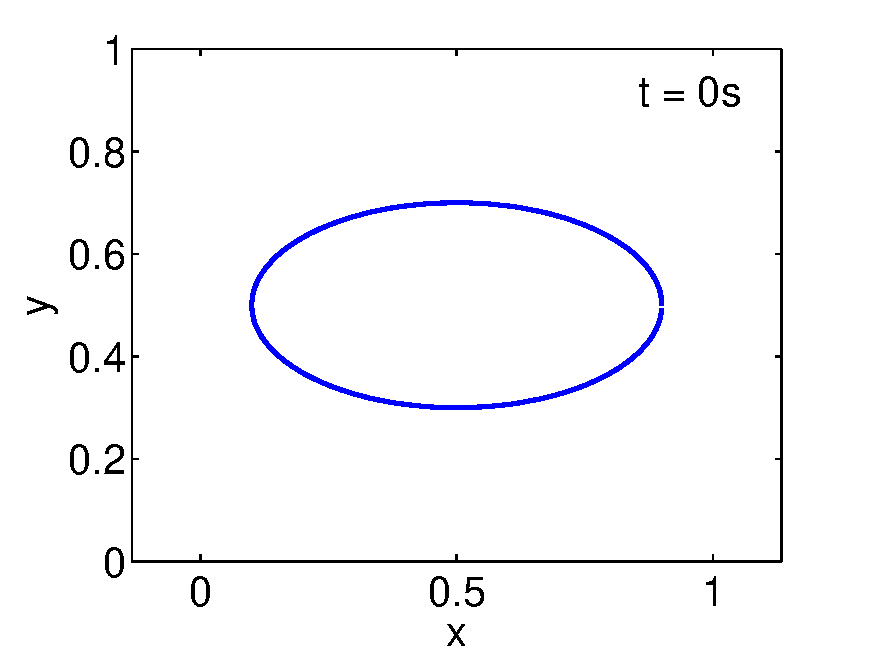
\includegraphics[width=.3\textwidth]{ellipse0000}\label{fig:ellipse0}}
	\subfigure[]{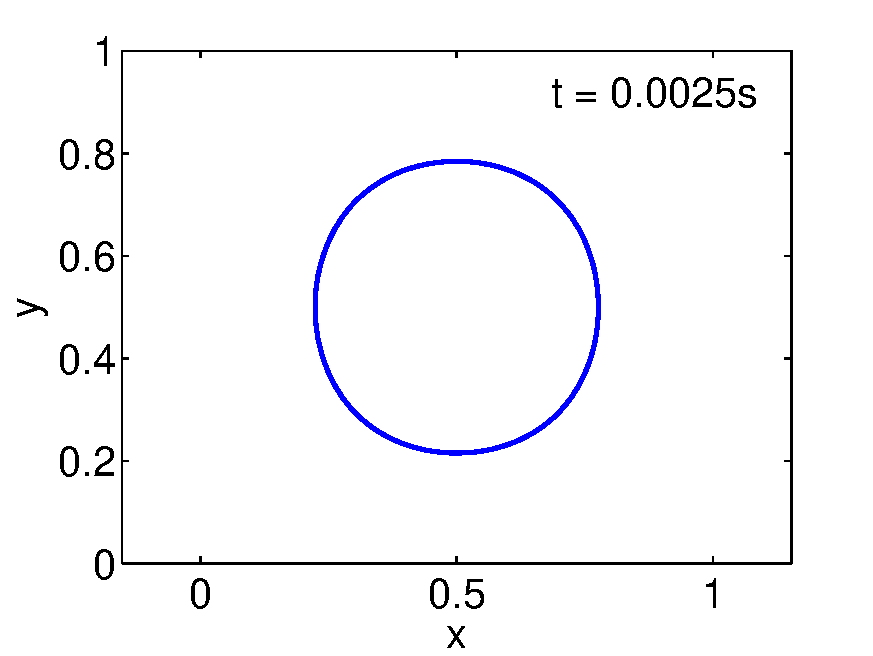
\includegraphics[width=.3\textwidth]{ellipse0025}\label{fig:ellipse1}}
	\subfigure[]{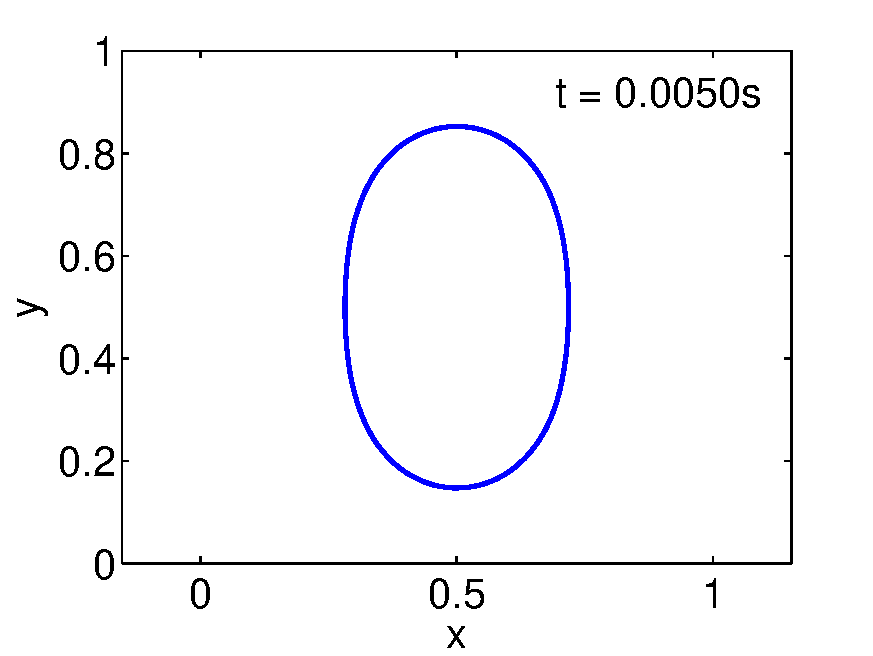
\includegraphics[width=.3\textwidth]{ellipse0050}\label{fig:ellipse2}}
  \subfigure[]{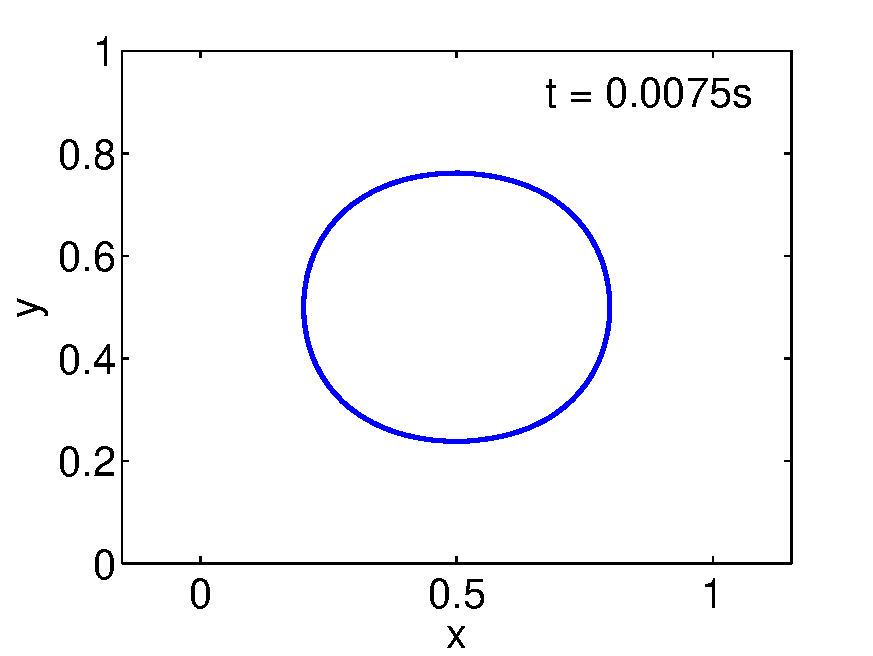
\includegraphics[width=.3\textwidth]{ellipse0075}\label{fig:ellipse3}}
	\subfigure[]{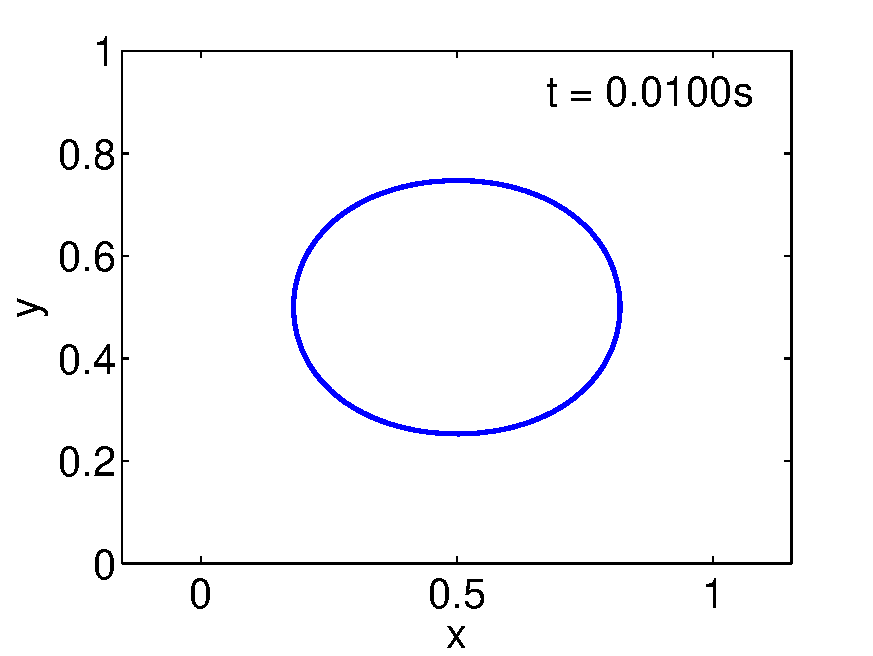
\includegraphics[width=.3\textwidth]{ellipse0100}\label{fig:ellipse4}}
	\subfigure[]{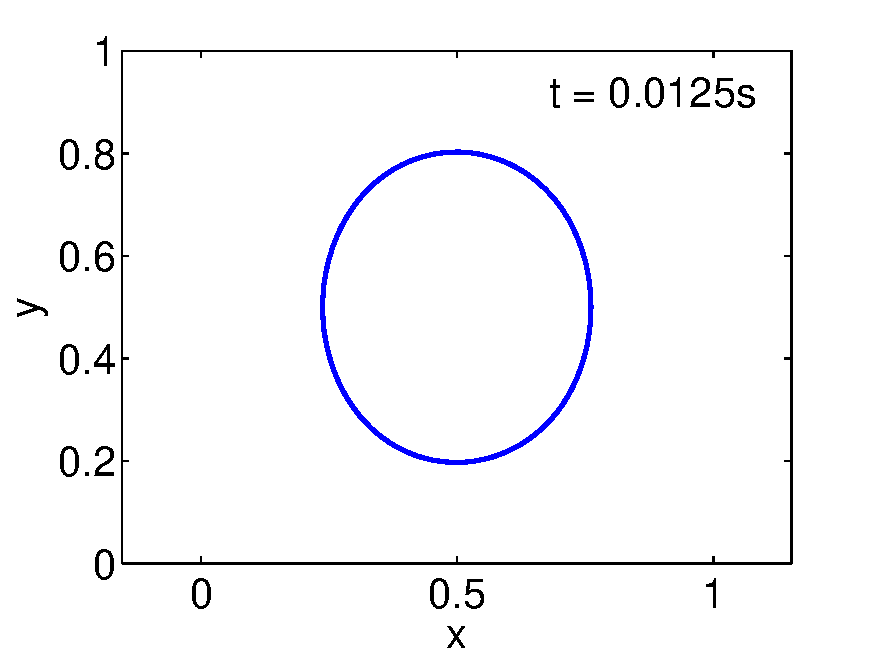
\includegraphics[width=.3\textwidth]{ellipse0125}\label{fig:ellipse5}}
  	\caption{Profiles of an elliptical membrane at different times. }
  	\label{fig:ellipseProfile}
\end{figure}

Before any IB simulation using MatIB, the solver first needs to be loaded. 
In the \mycode{EllipticalMembrane.m} script\footnote{The code assumes that \mycode{"cd ../../"} wil bring you to MatIB's root directory 
which is true when in the \mycode{"examples/Elliptical Membrane"} directory.}, this is accomplished using the commands:
\begin{lstlisting}
% Add PATH reference in order to run solver
addpath('../../solver/Peskin-TwoStep');
addpath('../../solver/utils');
\end{lstlisting}
which adds the solver folders to the top of Matlab's search path.
This allows the IB solver \mycode{solver/Peskin-TwoStep/IBSolver.m} and corresponding \mycode{util} functions to be called 
from within the Matlab script. Similarly, at the end of the Matlab script, we remove these folders from the search path 
using the commands:
\begin{lstlisting}
% Remove PATH reference to avoid clutter
rmpath('../../solver/Peskin-TwoStep');
rmpath('../../solver/utils');
\end{lstlisting}
By using this convention, it allows one to switch between IB solvers by simply changing the path name of the solver.

Once the script correctly links to the IB solver, the \mycode{IBSolver} function can be called 
with the following input parameters:
\begin{itemize}
\item \mycode{mu} : Dynamic viscosity $\mu$ in Navier-Stokes equation \eqref{eq:NSE}.
\item \mycode{rho}: Fluid density $\rho$ in Navier-Stokes equation \eqref{eq:NSE}.
\item \mycode{sigma} : Scalar spring constant $\sigma$ of the membrane defined in equation \eqref{eq:forceDensityDefinition}.
\item \mycode{L}: Scalar resting strain $L$ of the membrane defined in equation \eqref{eq:forceDensityDefinition}.

\item \mycode{IC\_U}, \mycode{IC\_V}: A function handle describing the initial velocity of the fluid $\bs{u}(\bs{x},0)$
						with the function profile:
						\begin{center}\mycode{ U = IC\_U(X,Y);}\end{center}
						Here, \mycode{X,\;Y} are matrices defining points on the Eulerian grid (created by Matlab's \mycode{meshgrid} function) and
						\mycode{U} is a matrix defining the $x$ component of the velocity field.
\item \mycode{IC\_ChiX},\;\mycode{IC\_ChiY}: Function handles returning the initial location of the membrane $\bs{X}(s,0)$
							with the function profile:
							\begin{center}\mycode{ ChiX = IC\_ChiX(S);}\end{center}
							The vector \mycode{S} corresponds to the discretized Lagrangian grid $s\in[0,1]$ with
							\mycode{ChiX} defining the $x$ component of the membrane position.
							
\item \mycode{Nx},\;\mycode{Ny} : Number of Eulerian grid points along the $x$- and $y$-axes.
\item \mycode{Lx},\;\mycode{Ly} : Length of domain along the $x$- and $y$-axes.
\item \mycode{Nb} : Number of grid points on the Lagrangian grid.
\item \mycode{NTime}: Number of time steps in the simulation.
\item \mycode{Tfinal}: The final time to compute the simulation to.

\item \mycode{ActionFun}: A function handle which is called after each time step with the function profile
							\begin{center}\mycode{ActionFun(dx, dy, dt, indT, X, Y, U, V, chiX, chiY, Fx, Fy);}\end{center}
							where 
							\begin{itemize}
								\item \mycode{dx},\;\mycode{dy}: The spatial step-size of the Eulerian grid.
								\item \mycode{dt}: The time-step used.
								\item \mycode{indT}: Index of current time step.
								\item \mycode{X},\;\mycode{Y}: Matrices defining spatial Eulerian grid points.
								\item \mycode{U},\;\mycode{V}: Matrices containing the current velocity field of the fluid on the Eulerian grid. 
								\item \mycode{chiX},\;\mycode{chiY}: Vectors containing the membrane's current position on the Lagrangian grid $s\in[0,1]$.
							\end{itemize}
\end{itemize}
When the function {\bf IBSolver} finishes running, it will return \mycode{[X, Y, S, U, V, chiX, chiY]} which are matrices of the Eulerian and Lagrangian grid,
the fluid velocity, and the membrane position at the last time step.
\newpage
In the \mycode{EllipticalMembrane.m} script, the IB solver is called as follows:
\begin{lstlisting}
% The number of grid points.
N = 32;
Nb = 3*N;

% Parameter values.
mu = 1;        % Viscosity.
sigma = 1e4;   % Spring constant.
rho = 1;       % Density.
rmin = 0.2;    % Length of semi-minor axis.
rmax = 0.4;    % Length of semi-major axis.
L = 0;         % Resting strain.

% Time step and final time.
Tfinal = .04;
dt = 5e-5;
NTime = floor(Tfinal./dt)+1;
dt = Tfinal ./ NTime;

% The initial velocity is zero.
IC_U = @(X,Y) zeros(size(X));
IC_V = @(X,Y) zeros(size(Y));

% The membrane is an ellipse.
IC_ChiX = @(S) 0.5 + rmax * cos(2*pi*S);
IC_ChiY = @(S) 0.5 + rmin * sin(2*pi*S);

% The action function.
Action = @( dx, dy, dt, indexT, X, Y, U, V, chiX, chiY, Fx, Fy)...
    PlotMembrane(X, Y, U, V, chiX, chiY, 1);

% Do the IB solve.
[X, Y, S, U, V, chiX, chiY] = ...
        IBSolver(mu, rho, sigma, L, IC_U, IC_V, IC_ChiX, IC_ChiY,...
        N, N, 1, 1, Nb, NTime, Tfinal, Action);
\end{lstlisting}
Note that there is a handy routine in the \mycode{solver/utils} folder called \mycode{PlotMembrane} 
which will plot the membrane's position and fluid velocity field.

\section{Acknowledgements}\label{sec:acknowledgements}

MatIB grew out of a course project where it has since been revised and used by numerous students at Simon Fraser University.
We would specifically would like to thank Professor John Stockie for his insight and feedback.

\newpage

\bibliography{citations}
\bibliographystyle{plain}



\end{document}


